\chapter{Weekly questions}

\section*{Week 10: A First Entry into Special Relativity}

\begin{question}
    How does the hyperboloid model work exactly, and what does it look like in Euclidean and Minkowski space?
\end{question}

\emph{Minkowski space(time)} is a combination of a three-dimensional Euclidean space and time into a four-dimensional manifold\footnote{\url{https://en.wikipedia.org/wiki/Minkowski_space}}. The isometry group of Minkowski space is the Poincaré group (or the Lorentz group, in a slightly more specific fashion). The isometry group of a metric space is the group of transformations under the action of which the metric remains invariant. The Minkowski space is endowed with an indefinite nondegenerate bilinear form called the Minkowski metric (or inner product) which yields the spacetime interval. This metric is \textbf{not} Riemannian as it is not positive-definite but only nondegenerate, which is why the Minkowski space is categorized as a pseudo-Riemannian manifold. This simply means that the Minkowski metric might vanish for nonzero vectors.

The \textit{Minkowski quadratic form} is defined as \footnote{\url{https://en.wikipedia.org/wiki/Hyperboloid_model}}
$$ Q(x_0, x_1, \ldots, x_n) = x_0^2 - x_1^2 - \ldots - x_n^2 $$
The polarization (a way of expressing an inner product in terms of a norm) of the Minkowski quadratic form is the Minkowski bilinear form $B$
$$ B(\vb{u}, \vb{v}) = \frac{1}{2} (Q(\vb{u} + \vb{v}) - Q(\vb{u}) - Q(\vb{v}))$$
The space $\real^{n+1}$ endowed with the Minkowski bilinear form is precisely the aforementioned Minkowski (pseudo-Riemannian) space. The choice of this specific bilinear form sets it apart from the traditional Euclidean space of dimension $n+1$ ($\mathbb{E}^{n+1}$) --- they are the \emph{same manifold} equipped with a \emph{different metric}.

All vectors $\vb{v}\in \real^{n+1}$ such that $Q(\vb{v}) = 1$ form an $n$-dimensional hyperboloid $S$ connecting of two sheets (the `future' sheet $S^{+} = \{\vb{v} \in S \mid v_0 > 0\}$ and the `past' sheet $S^{-} = \{\vb{v} \in S \mid v_0 < 0\}$ ). The hyperboloid model only considers the points on future sheet. A straight line in hyperbolic $n$-space is modeled as a geodesic on the hyperboloid. 

\begin{framed}
It is important to bear in mind the distinction between the Minkowski space and the hyperbolic space. Minkowski space is a flat space endowed with the Minkowksi metric. Hyperbolic space is a curved space.
\end{framed}

A \emph{Hyperbolic space} is a space with constant negative curvature.

The Lorentz group preserves the hyperboloid in Minkowski space.

\begin{question}
    How does the Special Relativity concept `interval' work in in finance?
\end{question}
The interval in Special Relativity is equal to the initial amount invested. Under Lorentzian transformations, the spacetime interval is conserved.

\begin{question}
    How do Lorentz transformations work in finance?
\end{question}
In general, Lorentz transformations are either boosts or rotations. In finance, boosts represent the action of compounding interest, or a `time march'. There is a very important difference that has to be kept in mind: in the `finance' Lorentzian space there is no time axis: the `special' dimension is reserved for capital instead. As a result, the boost operation has a time-varying argument.

\begin{question}
    How does the Minkowski metric arise from a simple compounding process?
\end{question}
\Cref{fig:compounding_example} exemplifies the compounding process with 5\% interest on an initial investment of \si{\money}1000. For now, it is immaterial what the compounding frequency is. The total value of the investment is decomposed into two parts, which will be called the `capital' and `yield' fractions. Every time the investment is `compounded', the following happens:
\begin{itemize}
    \item The interest rate acts on the amount of capital outstanding, the result of which adds to the current total yield.
    \item The interest rate acts on the current total yield, the result of which is added to the capital outstanding. This is sometimes called \textit{interest on interest} and lies at the very core of the compounding principle. If this action would not be present, the process reduces to simple interest.
\end{itemize}
Clearly, apart from the obvious symmetry, this decomposition is motivated by its intuitive interpretability. Much of what is to come in the dissertation hinges on this principle, which is why this example, obvious as it may seem, is important. 
\begin{figure}[ht!]
    \centering
    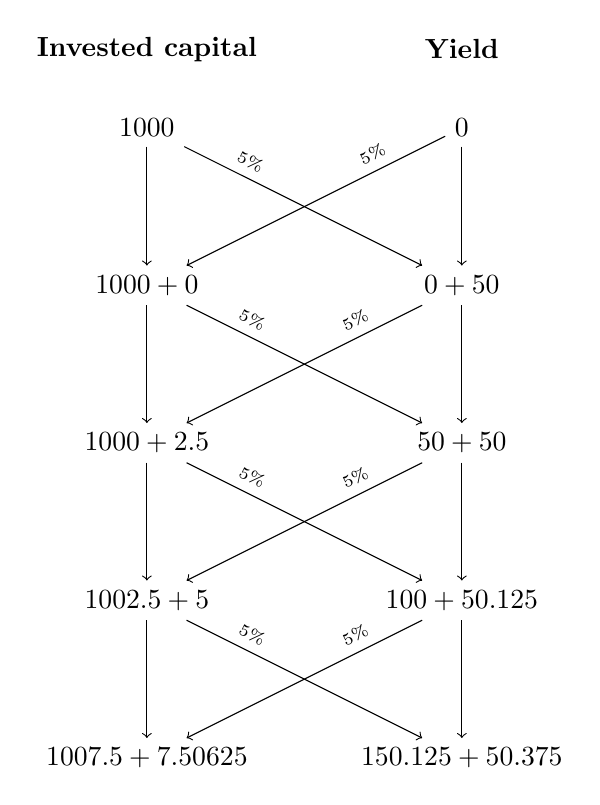
\begin{tikzpicture}
        \path (-2, 1)  node[fill=white, align=center]     {\textbf{Invested capital}};
        \path (2, 1)   node[fill=white, align=center]     {\textbf{Yield}};
        \path (-2, 0)  node[fill=white, align=center](x1) {1000};
        \path (2, 0)   node[fill=white, align=center](y1) {0};
        \path (-2, -2) node[fill=white, align=center](x2) {$1000 + 0$};
        \path (2, -2)  node[fill=white, align=center](y2) {$0 + 50$};
        \path (-2, -4) node[fill=white, align=center](x3) {$1000 + 2.5$};
        \path (2, -4)  node[fill=white, align=center](y3) {$50 + 50$};
        \path (-2, -6) node[fill=white, align=center](x4) {$1002.5 + 5$};
        \path (2, -6)  node[fill=white, align=center](y4) {$100 + 50.125$};
        \path (-2, -8) node[fill=white, align=center](x5) {$1007.5 + 7.50625$};
        \path (2, -8)  node[fill=white, align=center](y5) {$150.125 + 50.375$};
        
        \draw[->] (x1) -- (x2);
        \draw[->] (x2) -- (x3);
        \draw[->] (x3) -- (x4);
        \draw[->] (x4) -- (x5);
        
        \draw[->] (y1) -- (y2);
        \draw[->] (y2) -- (y3);
        \draw[->] (y3) -- (y4);
        \draw[->] (y4) -- (y5);
        
        \draw[->] (x1) -- node[near start, sloped, above] {\footnotesize{$_{5\%}$}} (y2);
        \draw[->] (x2) -- node[near start, sloped, above] {\footnotesize{$_{5\%}$}} (y3);
        \draw[->] (x3) -- node[near start, sloped, above] {\footnotesize{$_{5\%}$}} (y4);
        \draw[->] (x4) -- node[near start, sloped, above] {\footnotesize{$_{5\%}$}} (y5);
        \draw[->] (y1) -- node[near start, sloped, above] {\footnotesize{$_{5\%}$}} (x2);
        \draw[->] (y2) -- node[near start, sloped, above] {\footnotesize{$_{5\%}$}} (x3);
        \draw[->] (y3) -- node[near start, sloped, above] {\footnotesize{$_{5\%}$}} (x4);
        \draw[->] (y4) -- node[near start, sloped, above] {\footnotesize{$_{5\%}$}} (x5);
    \end{tikzpicture}
    \caption{Caption}
    \label{fig:compounding_example}
\end{figure}
Two approaches will be discussed that elegantly capture this process from a computational standpoint:  discrete LTI systems and hyperbolic-complex numbers. These methods are also closely related and essentially represent two sides of the same coin. The results that follow should therefore not come as surprising, though looking at them from different perspectives is certainly instructive.

\subsubsection*{Split-complex numbers}

[...]

\subsubsection*{Discrete dynamic system}
The translation from the process displayed in \cref{fig:compounding_example} is fairly obvious:
$$ 
    \vb{x}(k+1) = \mqty(1& \hanv \\ \hanv & 1)\vb{x}(k)\qq{with }\vb{x}(0) = \mqty(\ininv\\0)
$$
The solution of this autonomous system is given by:
$$
    \vb{x}(k) = \mqty(1& \hanv \\ \hanv & 1)^k\mqty(\ininv\\0)
$$
In order to motivate the further usage of the Lorentzian $n$-space, one can evaluate the Lorentzian norm of $\vb{x}(k)$ as follows:
$$
    \vb{x}(k)\circ\vb{x}(k) = \mqty(K & 0)\mqty(1& \hanv \\ \hanv & 1)^k\mqty(1 & 0\\0 & -1)\mqty(1& \hanv \\ \hanv & 1)^k\mqty(K\\0)
$$
Using eigenvalue decomposition of the system matrix
$$
    \vb{x}(k)\circ\vb{x}(k) = \vb{x}(0)^\top V\Lambda^k V^{-1} M V^{-1} \Lambda^k V \vb{x}(0)
$$
with
$$
    V = \mqty(-1 & 1 \\ 1 & 1) \quad \Lambda = \mqty(1 - \hanv & 0\\0 & 1 + \hanv)\quad M = \mqty(1 & 0 \\ 0 & -1)
$$
Straightforward computations yield then
$$
    \vb{x}(k)\circ\vb{x}(k) = K^2\qty(1 - \hanv^2)^k
$$
Clearly, this suggests that the Lorentzian norm of $\vb{x}(k)$ is \emph{almost} equal to $K^2$ apart from the multiplication by a number slightly smaller than 1 for reasonably small values of $\omega$. At this point one must realize that a discrete compounding process is always an approximation to the ideal case, which is why the Lorentzian norm is not exactly invariant under the transformation of the system matrix. Instead, let's subdivide a single time step into multiple compounding steps to achieve a better approximation:
$$ \vb{x}\circ\vb{x} = K^2 \lim_{n\to \infty} \qty(1 - \qty(\frac{\hanv}{n})^2)^{nk}$$
The limit on the right can be shown to be equal to 1\footnote{cf. notes}, which means that for continuous compounding, the Lorentzian norm is conserved.

\subsubsection*{Continuous LTI model properties}


\begin{question}
    What is the difference between the Poincaré group and the Lorentz group?
\end{question}
Quick and dirty: Poincaré group = Lorentz group + spacetime translations

The Poincaré group is sometimes said to contain both homogeneous and inhomogeneous Lorentz transformation.

\section{Week 15: Explore Ideas from Max}

\begin{question}
    How can we map interest movements in the Lorentz plane to the Smith chart?
\end{question}
\emph{Max' idea}: Map the asymptotes to the circumference of a circle, the capital axis to the diameter. Question is therefore: which mapping do we need to accomplish this? 
The traditional mapping of the Smith chart is:
$$ \Gamma = \frac{B\exp{-2\gamma l}}{A\exp{+2\gamma l}}$$
with $A$, $B$ constants

The mapping to project the interest movements in the Smith chart is a product of two Möbius transforms: 
$$ f_1(z) = z^2 \quad f_2(z) = \frac{z + 1}{z - 1}\qquad f(z) = (f_2 \circ f_1 )(z)  = \qty(\frac{z + 1}{z - 1})\qty(\frac{z + i}{z -i})$$
the former map is the traditional Smith chart.

How does this translate to a matrix?

\begin{question}
    Extra dimension for investments.
\end{question}